\documentclass{article}
\usepackage[utf8]{inputenc}
\usepackage[margin=1in]{geometry} % Ajusta los márgenes a 1 pulgada
\usepackage{graphicx}
\usepackage{listings}
\usepackage{xcolor}
\usepackage{hyperref}

\definecolor{codegreen}{rgb}{0,0.6,0}
\definecolor{codegray}{rgb}{0.5,0.5,0.5}
\definecolor{codepurple}{rgb}{0.58,0,0.82}
\definecolor{backcolour}{rgb}{0.95,0.95,0.92}

\lstdefinestyle{mystyle}{
    backgroundcolor=\color{backcolour},
    commentstyle=\color{codegreen},
    keywordstyle=\color{magenta},
    numberstyle=\tiny\color{codegray},
    stringstyle=\color{codepurple},
    basicstyle=\ttfamily\small,
    breakatwhitespace=false,
    breaklines=true,
    captionpos=b,
    keepspaces=true,
    numbers=left,
    numbersep=5pt,
    showspaces=false,
    showstringspaces=false,
    showtabs=false,
    tabsize=2
}

\lstset{style=mystyle}

\title{Convolutional Neural Networks – Lab 2}
\author{RUBEN MARTINEZ GONZALEZ}
\date{\today}

\begin{document}
    
    \maketitle
    
    
    \section{Introducción}
    \noindent
    En este informe, se presenta el trabajo realizado en el laboratorio 2 de Redes Neuronales Convolucionales.
    Se implementaron varias funciones relacionadas con el procesamiento de imágenes, incluyendo la aplicación de filtros Sobel, Laplacianos y detección de bordes.
    \noindent
    La solución se implementó en Python utilizando la biblioteca NumPy para el procesamiento de matrices y la biblioteca Matplotlib para la visualización de imágenes.
    La implementación está desplegada en un notebook de Google Colab, el cual se puede acceder a través del siguiente enlace:
    \texttt{%
        \href{https://colab.research.google.com/drive/1mX1coUf6sMoXGxgJmwHw3ILxTfAp5YeC#scrollTo=GDOnpOSTqdGX}{%
            Colab}%
    }
    
    
    \section{Funciones Implementadas}
    
    \subsection{Función sobelFiltering}\label{subsec:funcion-sobelfiltering}
    \noindent
    Esta función convoluciona una imagen con un filtro Sobel, que permite calcular la derivada de la intensidad de la imagen, pixel a pixel, en una dirección específica.
    La función toma como parámetros la matriz que almacena los datos de la imagen y el filtro Sobel vertical u horizontal a utilizar.
    
    \begin{lstlisting}[language=Python, caption={Implementación sobelfiltering},label={lst:sobelFiltering}]
def sobelFiltering(image, sobel_filter):

    kernel = np.flip(sobel_filter)
    height, width = image.shape
    filter_size = kernel.shape[0]
    filter_radius = filter_size // 2

    # Padded version of the image with zero-padding
    padded_image = np.pad(image, ((filter_radius, filter_radius), (filter_radius, filter_radius)), mode='constant')

    # Initialize array to store the filtered image
    filtered_image = np.zeros_like(image)

    # Iterate over each pixel in the image
    for i in range(height):
        for j in range(width):
            # Extract the neighborhood of the pixel from the padded image
            neighborhood = padded_image[i:i+filter_size, j:j+filter_size]
            # Apply the Sobel filters
            filtered_image[i, j] = np.sum(neighborhood * kernel)

    return filtered_image
    \end{lstlisting}
    
    \clearpage
    \noindent
    La implementación de esta función sigue la lógica descrita a continuación:
    \begin{itemize}
        \item Se inicializa el kernel invirtiendo el filtro Sobel que se recibe por parámetro y se obtienen las dimensiones de la imagen.
        \item Se crea una imagen con 'zero-padding' para poder aplicar el filtro en los bordes de la imagen.
        \item Se inicializa la imagen filtrada con ceros y las mismas dimensiones que la imagen original.
        \item Se itera sobre cada píxel de la imagen con padding y se extrae un vecindario de píxeles correspondiente.
        \item Se calcula un nuevo valor para cada pixel de la imagen filtrada aplicando el filtro Sobel al vecindario.
        \item Se retorna la imagen filtrada.
    \end{itemize}
    
    \noindent
    Todas las pruebas descritas en este documente se realizaron con la version a escalas de grises de la imagen a continuación.
    \texttt{%
        \href{https://drive.google.com/uc?id=1Vjzotd2ggul9GuD0adkf5KHCen6vQupK&authuser=0}{%
            Link de descarga:}%
    }
    \begin{figure}[!ht]
        \centering
        \caption{imagen\_original}
        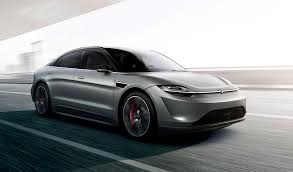
\includegraphics[width=0.5\textwidth]{img/carro}\label{fig:1}
    \end{figure}
    
    \noindent
    Se probó la función sobelFiltering con los siguientes filtros Sobel:
    \begin{itemize}
        \item Filtro Sobel en dirección 'X'
        \begin{lstlisting}[language=Python, caption={Filtro Sobel vertical},label={lst:sobelFiltersx}]
    Mx = np.array([
    [-1, 0, 1],
    [-2, 0, 2],
    [-1, 0, 1]
    ], dtype=float)
        \end{lstlisting}
        \item Filtro Sobel en dirección 'Y'
        \begin{lstlisting}[language=Python, caption={Filtros Sobel horizontal},label={lst:sobelFiltersy}]
    Mx = np.array([
    [-1, -2, -1],
    [ 0,  0,  0],
    [ 1,  2,  1]
    ], dtype=float)
        \end{lstlisting}
    \end{itemize}
    
    \clearpage
    \noindent
    Para ejecutar la prueba solo fue necesario llamar a la función sobelFiltering con la imagen y el filtro correspondiente.
    A modo complementario se desarrolló la función compare\_images para mostrar juntas la imagen original, la imagen filtrada y las diferencias entre ambas (resta de píxeles).
    
    \begin{lstlisting}[language=Python, caption={Ejecutando sobelFiltering},label={lst:compareImages}]
sobel_filtered_vertical_image = sobelFiltering(imagen_original, Mx)
compare_images(imagen_original,'Imagen Original', sobel_filtered_vertical_image, 'Filtro de Sobel vertical')
    \end{lstlisting}
    
    \begin{figure}[!ht]
        \centering
        \begin{subfigure}
            \centering
            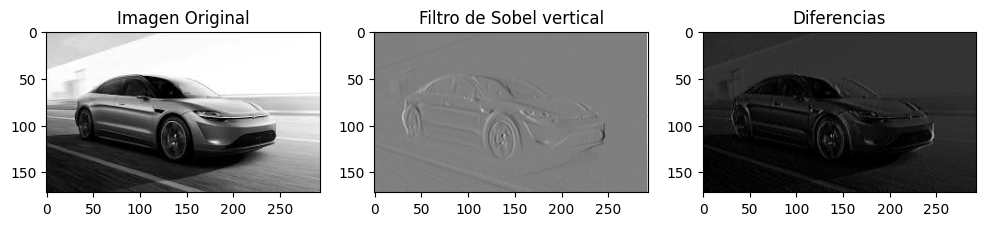
\includegraphics[width=\linewidth]{img/sobelx}
            \caption{ Resultado de aplicar el filtro Sobel en dirección 'X' a la imagen original.}
            \label{fig:sobelx}
        \end{subfigure}
        \begin{subfigure}
            \centering
            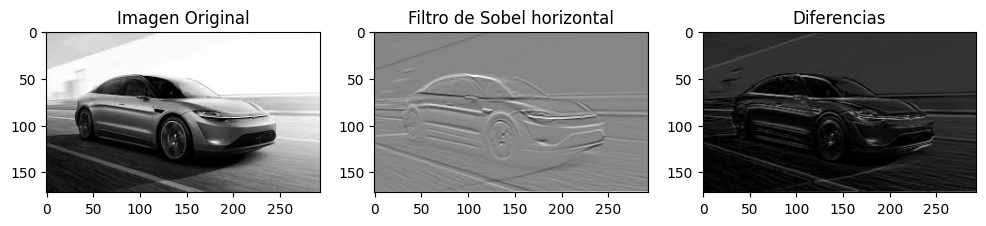
\includegraphics[width=\linewidth]{img/sobely}
            \caption{ Resultado de aplicar el filtro Sobel en dirección 'Y' a la imagen original.}
            \label{fig:sobely}
        \end{subfigure}
    \end{figure}
    
    \noindent
    \clearpage
    
    \subsection{Función laplacianFiltering}\label{subsec:funcion-laplacianfiltering}
    Esta función convoluciona una imagen con un filtro Laplaciano, que se utiliza para detectar cambios abruptos en la intensidad de los píxeles de una imagen.
    La función toma como parámetro la matriz que almacena los datos de la imagen.
    
    \begin{lstlisting}[language=Python, caption={Implementación laplacianFiltering},label={lst:laplacianFiltering}]
    def laplacianFiltering(image):

    laplacian_filter = np.array([
              [0,  1,  0],
              [1, -4,  1],
              [0,  1,  0]
             ], dtype=float)

    height, width = image.shape
    filter_size = laplacian_filter.shape[0]
    filter_radius = filter_size // 2

    # Padded version of the image with zero-padding
    padded_image = np.pad(image, ((filter_radius, filter_radius), (filter_radius, filter_radius)), mode='constant')

    # Initialize array to store the filtered image
    filtered_image = np.zeros_like(image)

    # Iterate over each pixel in the image
    for i in range(height):
        for j in range(width):
            # Extract the neighborhood of the pixel from the padded image
            neighborhood = padded_image[i:i+filter_size, j:j+filter_size]
            # Apply the Laplacian filter
            filtered_image[i, j] = np.sum(neighborhood * laplacian_filter)

    return filtered_image
    \end{lstlisting}
    
    \noindent
    La implementación de esta función sigue la prácticamente la misma lógica descrita anteriormente para la función sobelFiltering,
    excepto que en este caso se utiliza un filtro Laplaciano para aplicar la convolución.
    
    \noindent
    Se probó la función laplacianFiltering con la imagen utilizada anteriormente y se muestran los resultados a continuación.
    \begin{figure}[!ht]
        \centering
        \begin{subfigure}
            \centering
            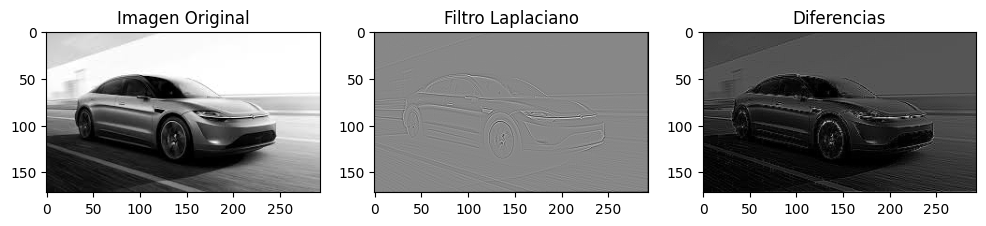
\includegraphics[width=\linewidth]{img/laplacian}
            \caption{ Resultado de aplicar el filtro Laplaciano a la imagen original.}
            \label{fig:laplacian}
        \end{subfigure}
    \end{figure}
    
    \subsection{Función edgeDetector}\label{subsec:funcion-edgedetector}
    Esta función aplica el kernel de gradiente en dirección 'X', el kernel de gradiente en dirección 'Y', calcula la magnitud del gradiente
    y realiza una umbralización de la magnitud del gradiente.
    La función toma tres parámetros: la matriz que almacena los datos de la imagen, un número que indica el tipo de kernel de gradiente a utilizar
    (se probaron dos tipos diferentes Sobel y Prewitt) y el valor de umbral.
    La función muestra la derivada en dirección 'X', la derivada en dirección 'Y' y los bordes umbralizados.
    Se implementó también un extra para mostrar en la imagen resultante formas de flecha representando la magnitud y dirección de los bordes umbralizados.
    
    La implementación de esta función se mostrará por partes para su mejor comprensión.
    \begin{itemize}
        \item
        Primero se aplica un suavizado a la imagen utilizando un filtro Gaussiano para reducir ruido y detalles innecesarios.
        (se reutiliza la función de suavizado averageFiltering implementada en el laboratorio 1)
        \begin{lstlisting}[language=Python, caption={Implementación edgeDetector - Suavisado},label={lst:edgeDetector1}]
# 1. Suavizado
gaussian_filter_matrix = np.array([
[1, 2, 1],
[2, 4, 2],
[1, 2, 1]
], dtype=float)
gaussian_filter_matrix /= np.sum(gaussian_filter_matrix)
smoothed_image = averageFiltering(image, gaussian_filter_matrix)
        \end{lstlisting}
        \item
        Luego se aplica el filtro de gradiente correspondiente (Sobel o Prewitt) a la imagen suavizada.
        \begin{lstlisting}[language=Python, caption={Implementación edgeDetector - Gradiente},label={lst:edgeDetector2}]
# 2. Realce
if type_gradient == 1:
    gradient_magnitude_image, filtered_vertical_image, filtered_horizontal_image = get_sobel_gradient_magnitude(smoothed_image)
elif type_gradient == 2:
    gradient_magnitude_image, filtered_vertical_image, filtered_horizontal_image = get_prewitt_gradient_magnitude(smoothed_image)
else:
    raise ValueError("Invalid type_gradient value. Choose 1 for Sobel or 2 for Prewitt.")
        \end{lstlisting}
        \begin{itemize}
            \item Se definieron complementariamente las funciones 'get\_sobel\_gradient\_magnitude' y
            \newline 'get\_prewitt\_gradient\_magnitude' para obtener la magnitud del gradiente.
            \begin{lstlisting}[language=Python, caption={Implementación get\_sobel\_gradient\_magnitude},label={lst:getSobelGradientMagnitude}]
def get_sobel_gradient_magnitude(image):
    Mx = np.array([
          [-1, 0, 1],
          [-2, 0, 2],
          [-1, 0, 1]
      ], dtype=float)

    My = np.array([
          [-1, -2, -1],
          [ 0,  0,  0],
          [ 1,  2,  1]
      ], dtype=float)

    sobel_filtered_vertical_image = sobelFiltering(imagen_original, Mx)
    sobel_filtered_horizontal_image = sobelFiltering(imagen_original, My)
    #               Magnitud =       √                        (df/dx)^2 + (df/dy)^2
    gradient_magnitude_image = np.sqrt(sobel_filtered_vertical_image**2 + sobel_filtered_horizontal_image**2)

    return gradient_magnitude_image, sobel_filtered_vertical_image, sobel_filtered_horizontal_image
            \end{lstlisting}
            \item Estas funciones aplican los filtros Sobel o Prewitt en dirección 'X' y 'Y' a la imagen original,
            calculan la magnitud del gradiente utilizando la fórmula $\sqrt{(df/dx)^2 + (df/dy)^2}$
            \item Se retorna la magnitud del gradiente y las derivadas en dirección 'X'(sobel\_filtered\_vertical\_image) y 'Y' (sobel\_filtered\_horizontal\_image).
            \item La función get\_prewitt\_gradient\_magnitude es similar a la anterior, pero utiliza los filtros Prewitt en lugar de los filtros Sobel.
            \begin{lstlisting}[language=Python, caption={Filtros prewitt},label={lst:Filtros prewitt}]
    Mx = np.array([
          [-1, 0, 1],
          [-1, 0, 1],
          [-1, 0, 1]
      ], dtype=float)

    My = np.array([
          [-1, -1, -1],
          [ 0,  0,  0],
          [ 1,  1,  1]
      ], dtype=float)
            \end{lstlisting}
        \end{itemize}
        \item A continuación se realiza una umbralización de la magnitud del gradiente estableciendo valor 255
        a los píxeles cuya magnitud sea mayor que el umbral y 0 en caso contrario.
        La representación resultante se almacena en la variable thresholded\_edges.
        \begin{lstlisting}[language=Python, caption={Implementación edgeDetector - Umbralización},label={lst:edgeDetector3}]
# 3. Umbralización
thresholded_edges = np.where(gradient_magnitude_image > threshold, 255, 0)
        \end{lstlisting}
        
        \item A continuación se dibujan flechas en la imagen resultante para representar la magnitud y dirección de los bordes umbralizados.
        Para ello realizaron los siguientes calculos adicionales:
        \begin{itemize}
            \item se obtuvieron puntos aleatorios en la zona central de la imagen.
            La cantidad de puntos se estableció en num\_arrows = 10.
            Para ello se Implementó la función get\_edge\_points.
            \begin{lstlisting}[language=Python, caption={Implementación edgeDetector - edge\_points},label={lst:edgeDetector4}]
     # 4. Dibujar flechas en los bordes umbralizados
    edge_points = get_edge_points(thresholded_edges, num_arrows = 10)
            \end{lstlisting}
            \item La función get\_edge\_points recibe como parámetro la imagen umbralizada y la cantidad de puntos a seleccionar.
            Se encarga de obtener los puntos en los que la imagen umbralizada tiene valor 255 y seleccionar solo los puntos en la zona central de la imagen.
            Se acotó la zona central de la imagen con un margen del 25\% desde el borde de la imagen por conveniencia para disminuir la posibilidad
            de que al pintar las flechas estas se salgan de la imagen.
            \begin{lstlisting}[language=Python, caption={Implementación get\_edge\_points},label={lst:getEdgePoints}]
def get_edge_points(thresholded_edges, num_arrows = 10):
    edge_points = np.argwhere(thresholded_edges == 255)
     # Obtener límites de la zona central
    h, w = thresholded_edges.shape
    margin = int(min(h, w) * 0.25)  # Margen del 25% desde el borde de la imagen
    min_x = margin
    max_x = w - margin
    min_y = margin
    max_y = h - margin

    # Seleccionar puntos aleatorios de la zona central
    edge_points = [point for point in edge_points if min_x < point[1] < max_x and min_y < point[0] < max_y]
    np.random.shuffle(edge_points)
    edge_points = edge_points[:num_arrows]  # Tomar solo algunos puntos para las flechas

    return edge_points
            \end{lstlisting}
            \item Se obtuvo la dirección del gradiente en cada punto de la imagen umbralizada utilizando la función np.arctan2.
            La función np.arctan2 recibe como parámetros las derivadas en dirección 'X' y 'Y' y retorna el ángulo correspondiente.
            Los ángulos se almacenaron en la variable gradient\_direction\_image.
            \begin{lstlisting}[language=Python, caption={Implementación edgeDetector - gradient\_direction},label={lst:edgeDetector5}]
gradient_direction_image = np.arctan2(filtered_horizontal_image, filtered_vertical_image)
            \end{lstlisting}
            
            \item
            \item Finalmente se dibujaron las flechas en la imagen umbralizada recorriendo los puntos obtenidos aleatoriamente en el paso anterior,
            calculando las coordenadas finales de la flecha y utilizando la función plt.arrow de la biblioteca Matplotlib.
            Las coordenadas finales de la flecha se calcularon con las fórmulas:
            \begin{itemize}
                \item dx = magnitud * np.cos(dirección)
                \item dy = magnitud * np.sin(dirección)
            \end{itemize}
            La magnitud se dividió por 10 a conveniencia para que las flechas se escalen adecuadamente en la imagen.
            \begin{lstlisting}[language=Python, caption={Implementación edgeDetector - Dibujar flechas},label={lst:edgeDetector6}]
  for point in edge_points:
    y, x = point
    magnitude = gradient_magnitude_image[y, x]/10
    direction = gradient_direction_image[y, x]

    # Calcular las coordenadas finales de la flecha
    dx = magnitude * np.cos(direction)
    dy = magnitude * np.sin(direction)

    plt.arrow(x, y, dx, dy, color='red', head_width=4, head_length=8)
            \end{lstlisting}
        
        \end{itemize}
        
        \clearpage
        \item Finalmente se muestran los resultados obtenidos en 4 subfiguras que contienen:
        \begin{itemize}
            \item La derivada en dirección 'X'
            \item La derivada en dirección 'Y'
            \item Los bordes umbralizados
            \item Las flechas que representan la magnitud y dirección de los bordes umbralizados.
        \end{itemize}
        \begin{lstlisting}[language=Python, caption={Implementación edgeDetector - Mostrar resultados},label={lst:edgeDetector7}]
plt.subplot(2, 2, 1)
plt.imshow(filtered_vertical_image, cmap='gray')
plt.title('Derivative in x direction')

plt.subplot(2, 2, 2)
plt.imshow(filtered_horizontal_image, cmap='gray')
plt.title('Derivative in y direction')


plt.subplot(2, 2, 3)
plt.imshow(thresholded_edges, cmap='gray')
plt.title(f'Umbralización (Threshold = {threshold})')

plt.subplot(2, 2, 4)
plt.imshow(thresholded_edges, cmap='gray')
plt.title(f'Arrow shapes magnitude and directions')
        
        \end{lstlisting}
    \end{itemize}
    
    \noindent
    Se probó la función edgeDetector con la imagen utilizada anteriormente y se muestran los resultados a continuación.
    \begin{figure}[!ht]
        \centering
        \begin{subfigure}
            \centering
            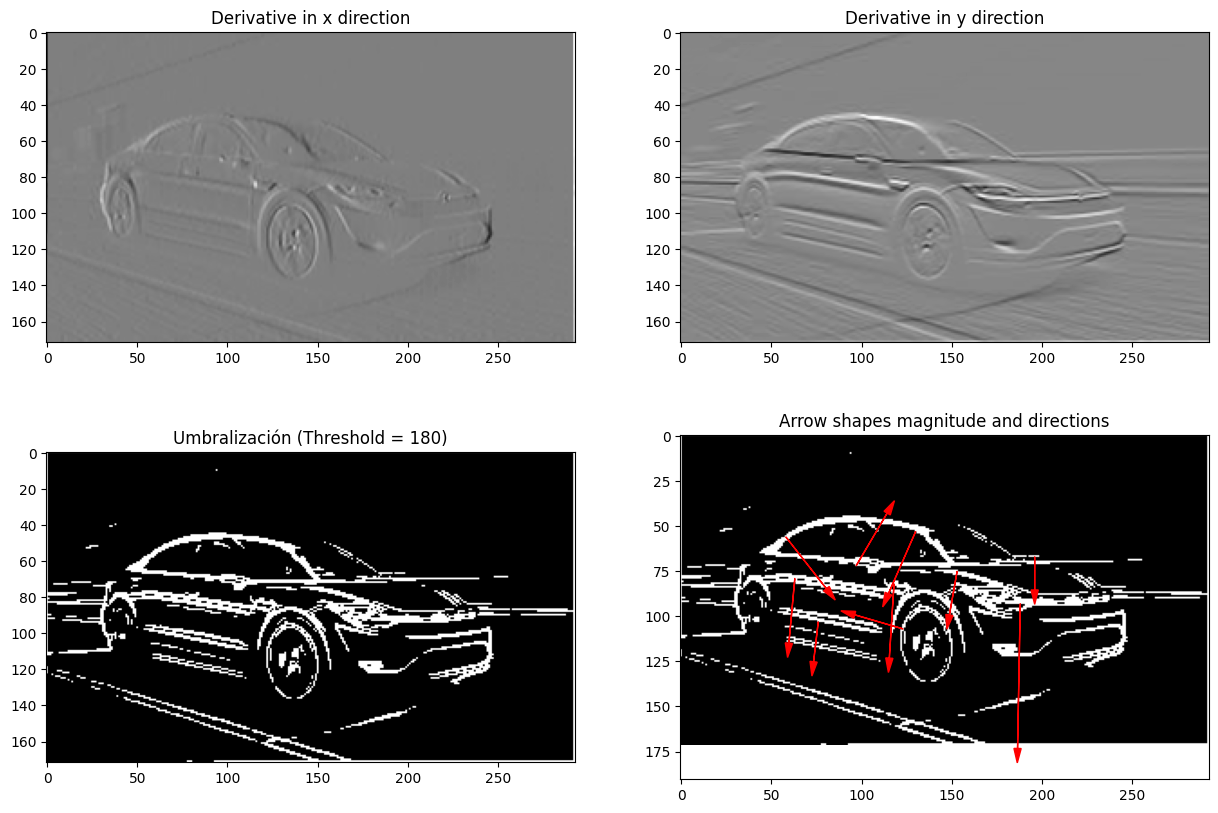
\includegraphics[width=\linewidth]{img/bordeSobel}
            \caption{ Resultado de aplicar el detector de bordes con filtro Sobel y umbral 180.}
            \label{fig:edgesso}
        \end{subfigure}
        \begin{subfigure}
            \centering
            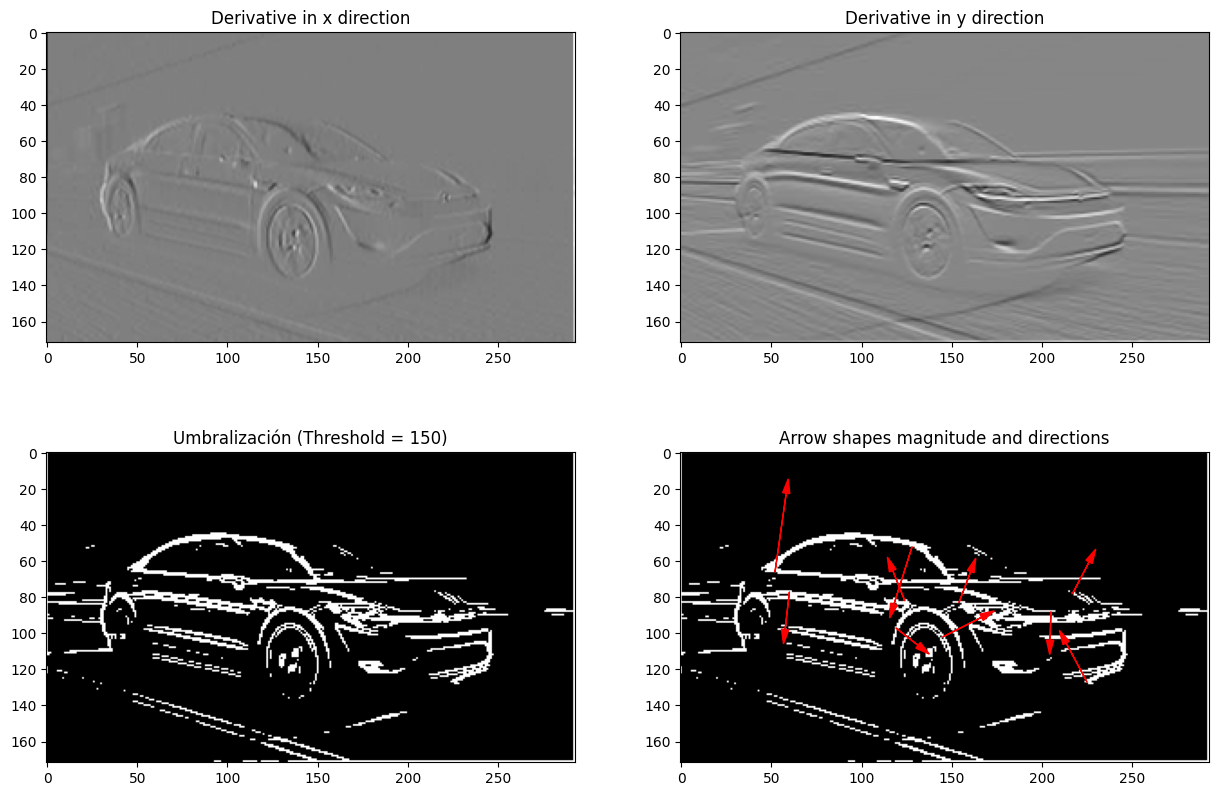
\includegraphics[width=\linewidth]{img/bordePrewitt}
            \caption{ Resultado de aplicar el detector de bordes con filtro Prewitt y umbral 180.}
            \label{fig:edgespw}
        \end{subfigure}
    \end{figure}
    
    \clearpage
    \section{Conclusiones}
    En esta práctica se implementaron varias funciones para el procesamiento de imágenes, incluyendo filtros Sobel y Laplacianos,
    así como la detección de bordes utilizando el kernel de gradiente en dirección 'X' y 'Y'.
    Se logró aplicar estos filtros y detectores de bordes a una imagen a escala de grises y se obtuvieron resultados satisfactorios.
    Estas técnicas son fundamentales en el campo de la visión por computadora y son ampliamente utilizadas en aplicaciones de reconocimiento de objetos y segmentación de imágenes.
    

\end{document}
